\section{Durchführung}
\label{sec:Durchführung}

\subsection{Bestimmung der Zeitkonstante des RC-Kreises mithilfe der Entladekurve} % (fold)
\label{sub:Entladekurve_durch}
Zur Bestimmung der Zeitkonstante wird die Schaltung in \autoref{fig:Zeitkonstante_durch} aufgebaut,
wobei vom Oszilloskop die Kondensatorspannung $U_C(t)$ in Abhängigkeit von der Zeit angezeigt wird.
\begin{figure}[H]
    \centering
    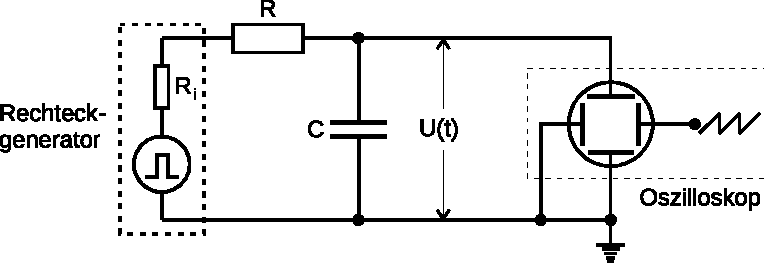
\includegraphics[width=0.69\textwidth]{build/Abb_3.pdf}
    \caption{Schaltbild zur Bestimmung der der Zeitkonstante.\cite{v353}}
    \label{fig:Entladekurve_durch}
\end{figure}
\noindent Mit dem Rechteckgenerator wird eine Rechteckspannung mit einer Frequenz angelegt, sodass sich während der Aufzeichnungszeit die Kondensatorspannung $U_C(t)$ um den Faktor $5$ bis $10$ ändert.
Nachdem das Oszilloskop richtig eingestellt wird, sodass eine Entladekurve angezeigt wird, werden $12$ Werte abgelesen und in eine Tabelle eingetragen. 
% subsection Bestimmung der Zeitkonstanten des RC-Kreises (end)
\subsection{Bestimmung der frequenzabhängigen Amplitude und Phasenverschiebung} % (fold)
\label{sub:Freque_A&P_durch}
\noindent Die Schaltung aus \autoref{fig:Zeitkonstante_durch} wird so verändert, dass das Oszilloskop nun ein Zweikanal-Oszilloskop ist.
Es wird eine Sinusspannung angelegt und die Frequenz von Hand variiert.
Gemessen wird in einem Bereich von $\qty{20}{\hertz}$ bis $\qty{20000}{\hertz}$ und pro Zehnerpotenz werden $5$ Werte genommen.
Zu jedem Messpunkt werden die Frequenz, die Amplitude und der Abstand der Extrempunkte der beiden Kurven abgelesen und in eine Tabelle eingetragen.
\begin{figure}[H]
    \centering
    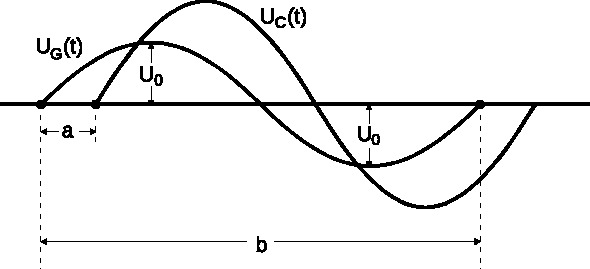
\includegraphics[width=0.69\textwidth]{build/Abb_7_edit.pdf}
    \caption {Messung der Phasenverschiebung zwischen zwei Spannungen.\cite{v353}}
    \label{fig:Freque_A&P_durch}
\end{figure}
% subsection Bestimmung der frequenzabhängigen Amplitude und Phasenverschiebung (end)
\subsection{Ein RC-Kreis als Integrator} % (fold)
\label{sub:Integrator_durch}
Am Generator wird eine Frequenz von $\qty{800}{\hertz}$ eingestellt.
Der Reihe nach werden dann eine Sinus-, Rechteck- und Dreickspannung angelegt.
Auf dem Bildschirm sollen nun die integrierte und die zu integrierende Spannung zu sehen sein.
Anschließend wird von jeder Spannung ein Bild gemacht.

% subsection Ein RC-Kreis als Integrator (end)
